%\setchapterimage{bandeau}
\chapter*{Application \arabic{cptApplication} :\\ 
Liaisons équivalentes -- \ifprof Corrigé \else Sujet \fi}
\addcontentsline{toc}{section}{Application \arabic{cptApplication} : Liaisons équivalentes -- \ifprof Corrigé \else Sujet \fi}

\iflivret \stepcounter{cptApplication} \else
\ifprof  \stepcounter{cptApplication} \else \fi
\fi

\setcounter{question}{0}
\marginnote{D'après P. Dupas.}
%\marginnote[1cm]{
%\UPSTIcompetence[2]{B2-10}
%}
%\begin{marginfigure}
%\centering
%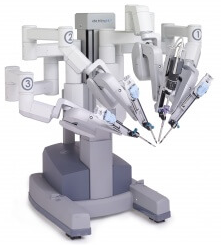
\includegraphics[width=4cm]{fig_00}
%\end{marginfigure}



\subsection*{Liaisons en parallèle}

\question{Déterminer la liaison équivalente des liaisons suivantes.}
\begin{multicols}{2}
\begin{center}
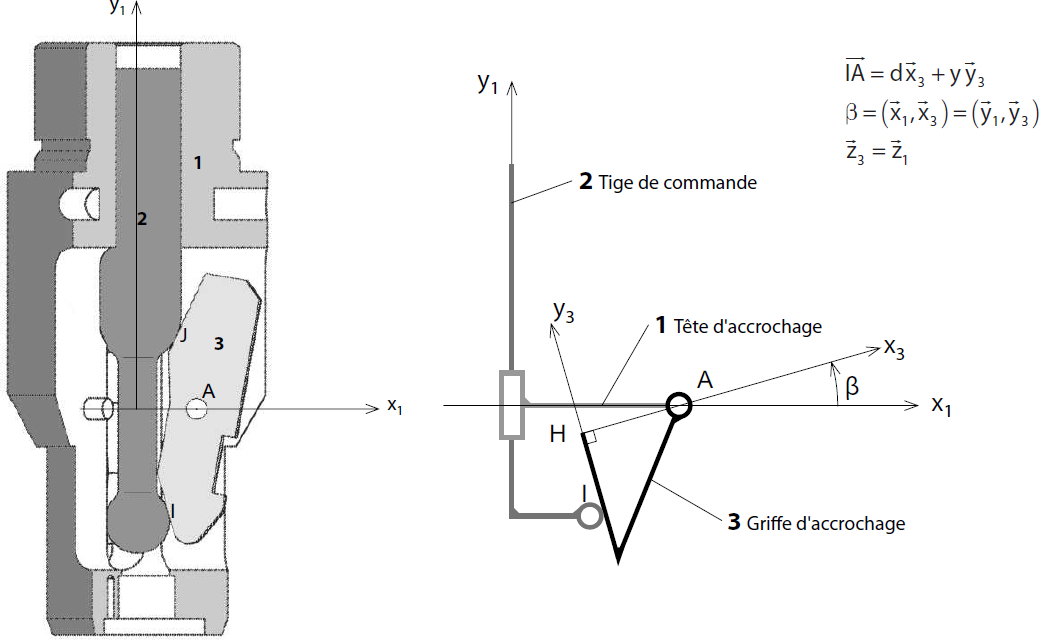
\includegraphics[width=.8\linewidth]{fig_01.png}
\end{center}

\begin{center}
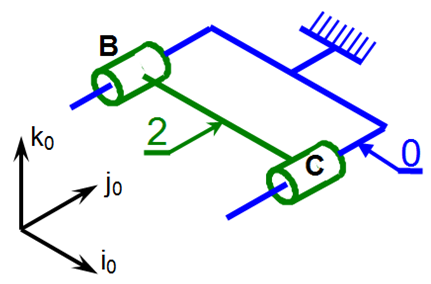
\includegraphics[width=.8\linewidth]{fig_02.png}
\end{center}

\begin{center}
\rotatebox{90}{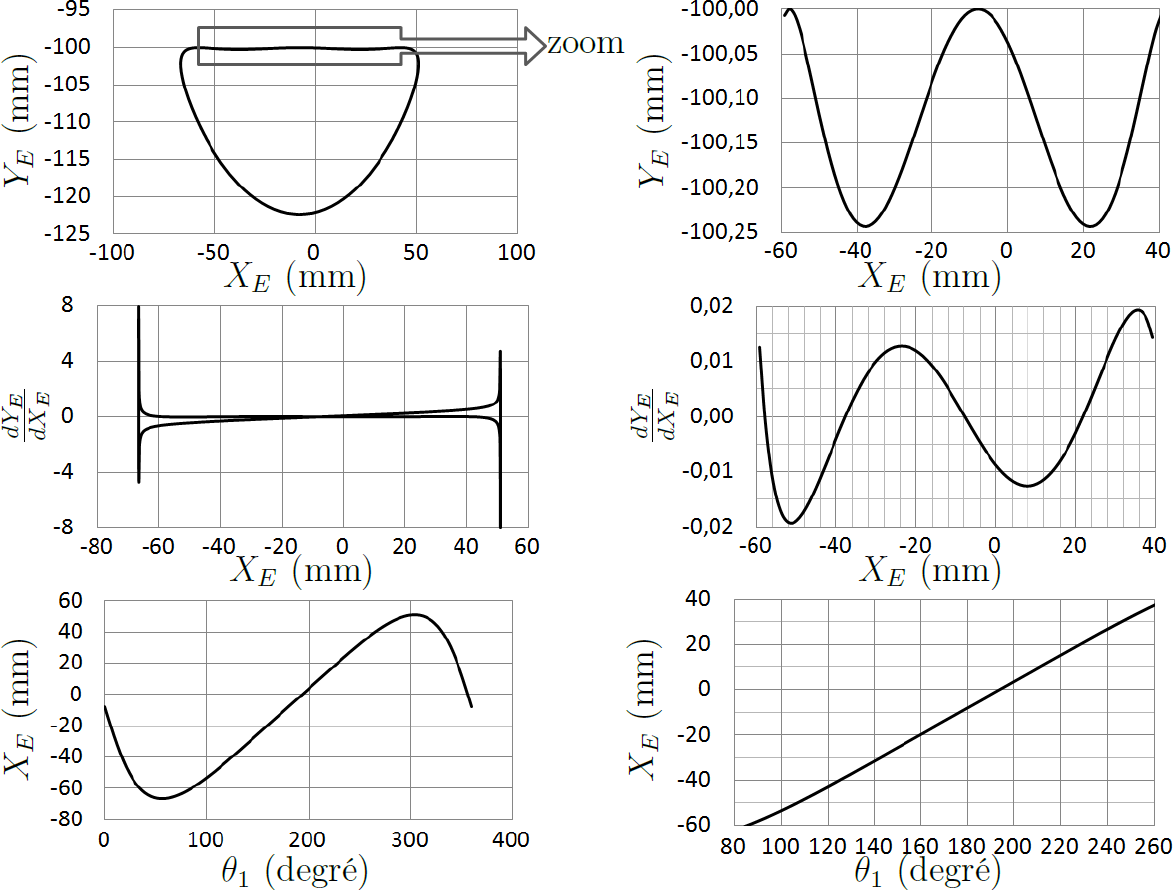
\includegraphics[width=.6\linewidth]{fig_03.png}}
\end{center}

\begin{center}
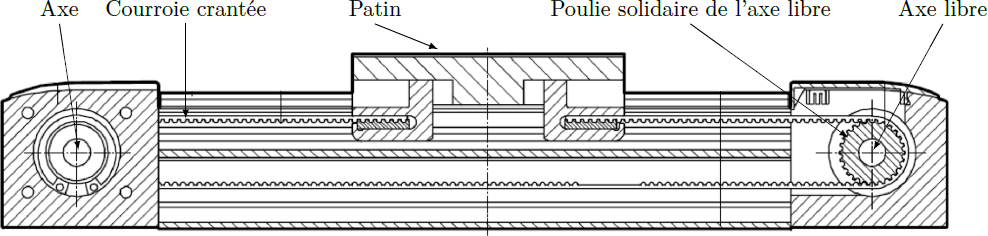
\includegraphics[width=.8\linewidth]{fig_04.png}
\end{center}

\begin{center}
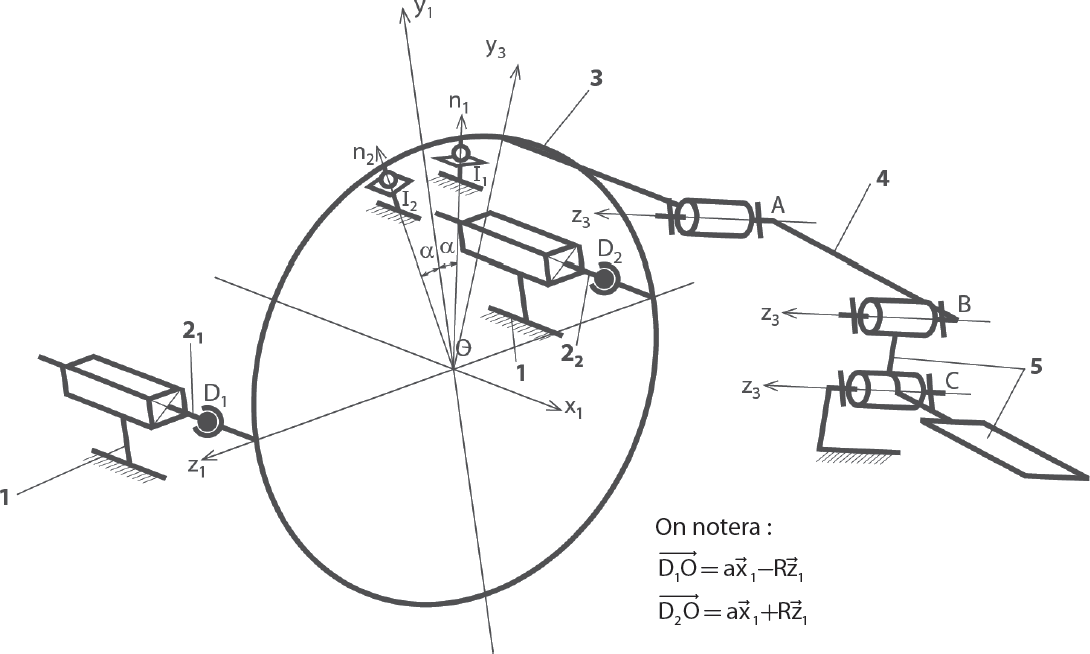
\includegraphics[width=.8\linewidth]{fig_05.png}
\end{center}

\begin{center}
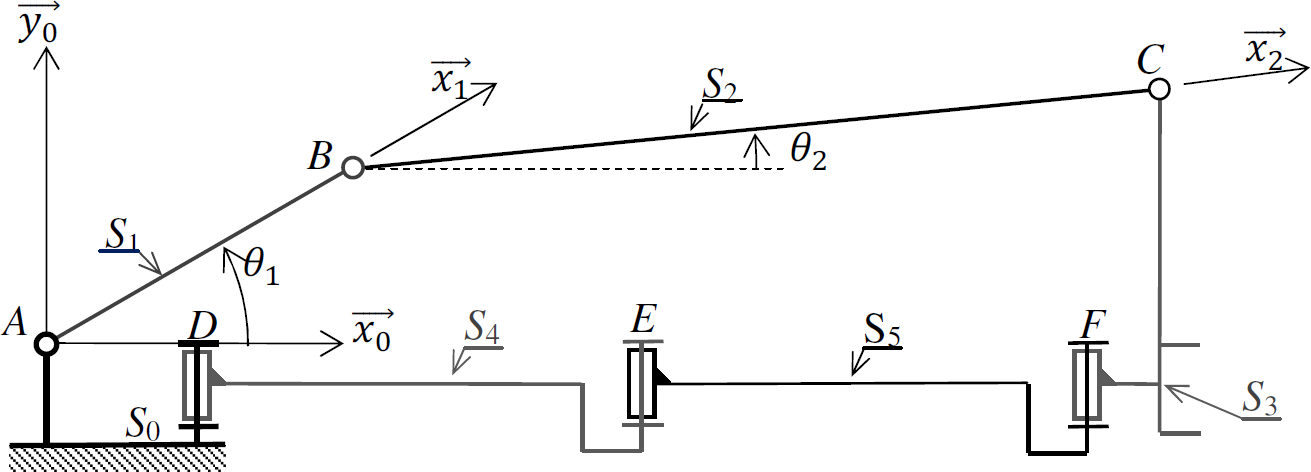
\includegraphics[width=.8\linewidth]{fig_06.png}
\end{center}

\begin{center}
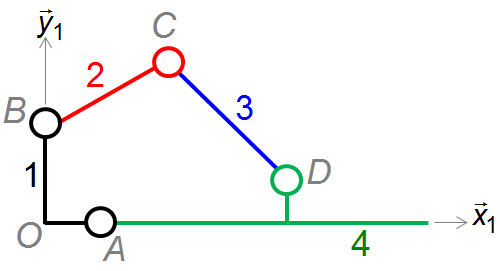
\includegraphics[width=.8\linewidth]{fig_07.png}
\end{center}

\begin{center}
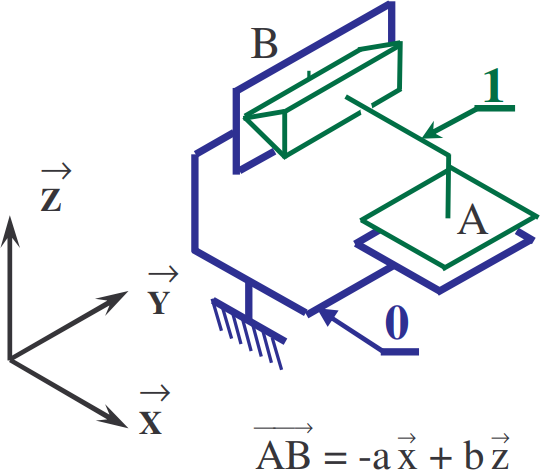
\includegraphics[width=.8\linewidth]{fig_08.png}
\end{center}



\begin{center}
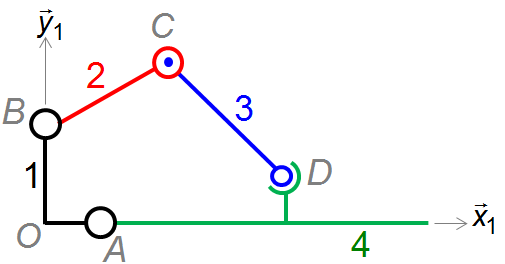
\includegraphics[width=.5\linewidth]{fig_09.png}
\end{center}

\begin{center}
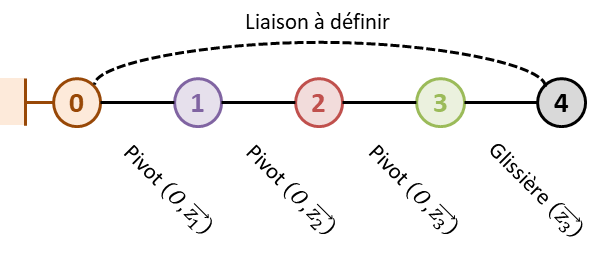
\includegraphics[width=.8\linewidth]{fig_10.png}
\end{center}

\end{multicols}
\subsection*{Liaisons en série}

\question{Déterminer la liaison équivalente des liaisons suivantes.}

\begin{multicols}{2}
\begin{center}
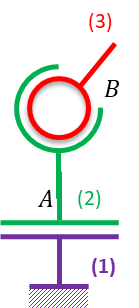
\includegraphics[width=.3\linewidth]{fig_11.png}
\end{center}
\begin{center}
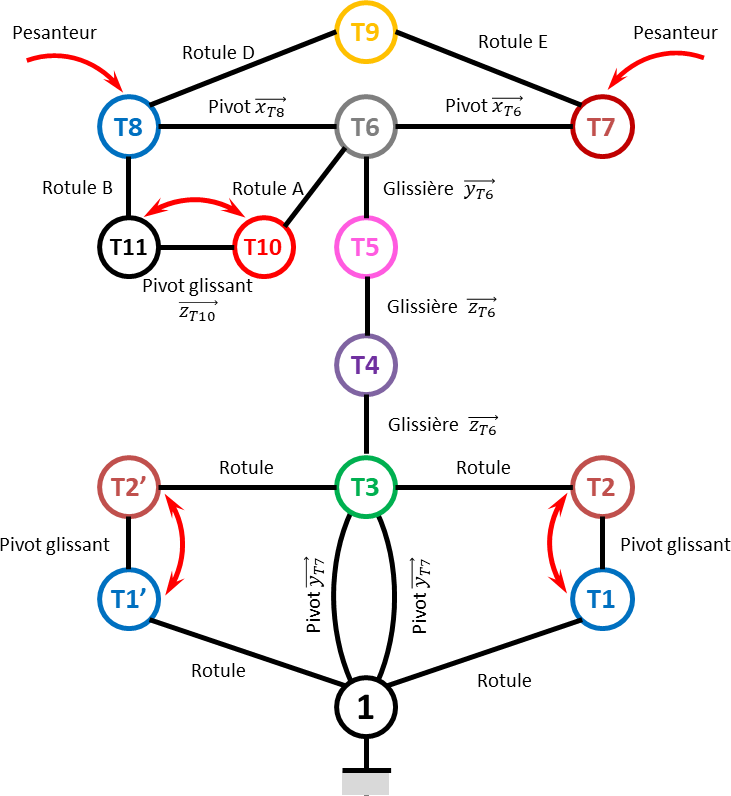
\includegraphics[width=.25\linewidth]{fig_12.png}
\end{center}
\end{multicols}
